 \pagebreak
\subsection{Diagrama esquem\'atico del circuito}
Se presentan el diagrama esquem\'atico del circuito electr\'onico y las vistas de la baquelita que se elabor\'o.

 \begin{figure}[!htbp]
 \centering
 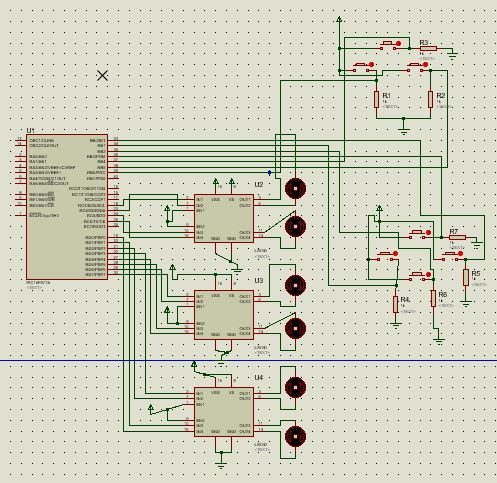
\includegraphics [scale=0.5]
 {./img/seaperch_schematic.png}
 \caption{Diagrama esquem\'atico del circuito.}
 \end{figure}

  \begin{figure}[!htbp]
 \centering
 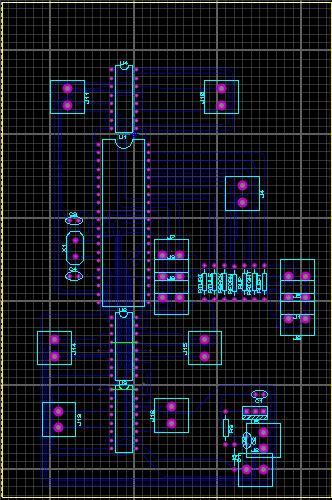
\includegraphics [scale=0.5]
 {./img/seaperch_pcb.png}
 \caption{Layout del PCB.}
 \end{figure}

  \begin{figure}[!htbp]
 \centering
 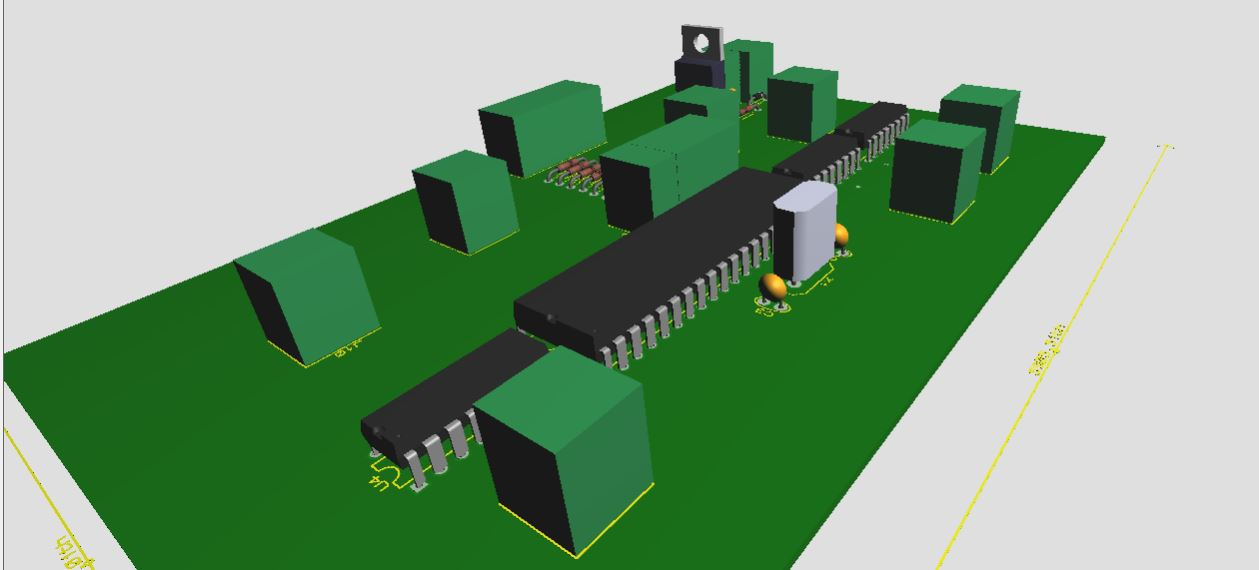
\includegraphics [scale=0.35]
 {./img/seaperch_pcb_3d_01.png}
 \caption{Vista 3D del PCB.}
 \end{figure}

   \begin{figure}[!htbp]
 \centering
 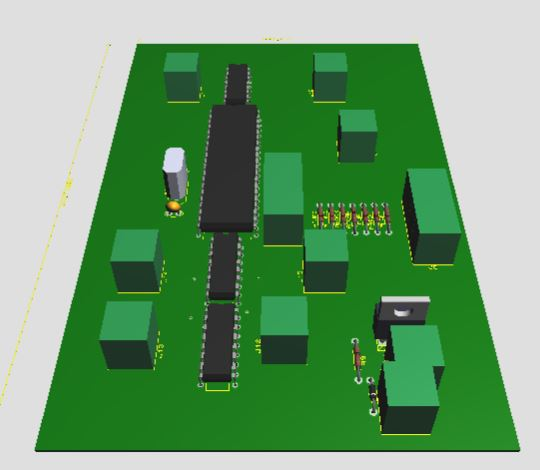
\includegraphics [scale=0.45]
 {./img/seaperch_pcb_3d_02.png}
 \caption{Vista 3D del PCB.}
 \end{figure}

 \pagebreak

